

\documentclass{beamer}

\usepackage[utf8]{inputenc} % permite a escrita com acento
\usepackage{default}
\usetheme{CambridgeUS}


\usepackage{listings}       % Pacote Listings para inclusão de codigo-fonte no documento
\usepackage{hyperref}	% Pacote para criar links

\useoutertheme{infolines}

\title[Introdução ao Flex e Bison]{Introdução ao Flex e Bison}
\author[Lucas, André, George, Luis, Walderi]
       {Lucas Begnini Costa // André Moreira // George Lucas Gomes // Luiz Sergio // Walderi Filho}
			
	\institute[UEA]{Universidade do Estado do Amazonas}
\date{\today}

\begin{document}  % Inicio dos slides
%Slide Inicial - Inicio

\begin{frame}[plain] % Frame significa Slide, entao toda vez que
    \titlepage   	% tiver begin e end Frame significa que o slide 
		    % tem tudo oq há entre os  2
	
            \begin{figure} 	%para inserir figura basta fazer o mesmo que frame
            \centering		% Significa que a figura está centralizada no slide
            
\includegraphics[scale=0.41]{simbolouea} %A figura pra ser add assim tem q ta no diretorio do tex
            \end{figure}
	\date{\today}  		% Insere a data da compilação
\end{frame}			% Fim do primeiro slide

\frame{\titlepage}

% Slide Inicial - Final
%Slide 02 - Inicio


\begin{frame}
  \frametitle{Sumário}		% Insere o titulo do Slide
  \tableofcontents		% Insere tudo o conteudo existente nos slides
\end{frame}			% Processo feito automaticamente


%Slide 02 - Fim
%Slide 03 - Inicio
\section{Introdução}		% Delimito o titulo da nova sessao, ou seja, capitulo
\begin{frame} 			% Inicializo o slide 
\frametitle{Introdução}
  Este trabalho tem como intuito apresentar a construção de uma calculadora	% Assunto que irá 
 que será utilizada através de linha de comando e interpretada através de:	%ficar dentro do slide
 
    \begin{itemize} 				% Assim inicializa os itens 
     \item<1-> Flex - Analisador léxico    	% esse ``1'' dentro de < .. > 
     \item<2-> Bison - Analisador semântico	 % Simboliza a ordem que será mostrado os itens 
    \end{itemize}				% Finaliza os itens 
  Para apresentar a calculadora será necessário uma breve apresentação a respeito de
 Flex e Bison

\end{frame}			% Finalizo o slide

\section{FLEX}			%Inicio da sessão do flex
%Slide 04 - Inicio
\begin{frame}
\frametitle{FLEX}
  Como falado anteriormente o Flex é uma ferramenta para criação de analisadores Léxicos que
 procura padrões de escrita através de expressões regulares definidas dentro dos analisadores léxicos.
  Como resultado, depois da compilação do arquivo flex feito, é gerado um arquivo em C que valida
 todas as expressões regulares definidas no arquivo que passará pelo Flex
 
\end{frame}

%Slide 05 - Inicio
\subsection{Instalando Flex no Linux}
\begin{frame}
\frametitle{Instalando Flex no  Linux}
	Antes de fazer qualquer coisa para criação do arquivo flex é necessário inicialmente a instalação do 
compilador flex no sistema operacional, no caso utilizado foi o Linux Ubuntu 13.04.
	Para instalação é necessário abrir o terminal e por linha de comando digitar: 
			\\ \$ sudo apt-get install flex
\end{frame}



%Slide 06- Inicio
\subsection{Criando um arquivo para o Flex}
\begin{frame}
\frametitle{Criando um arquivo para o Flex}

  Para a criação de um arquivo para o flex não é necessário nenhuma extensão especifica, podendo ser 
 o que o desenvolvedor quiser, mas como um ato de boa pratica de programação, padronizou-se como .lex ou 
 .l para melhor distinguir de outros arquivos.

\end{frame}
%Slide 07 - Inicio
\begin{frame}
\frametitle{Criando um arquivo para o Flex}

  Dentro do programa há duas partes, separado por "\%\%" dividindo o programa em duas partes: %%Tem q ter o \ porque % é um caracter reservado do latex
A primeira para delimitação das expressões regulares que serão consideradas, e a segunda as ações que serão
tomadas caso encontre as expressões regulares definidas anteriormente.Como podemos ver no exemplo seguinte:
 \href{https://github.com/Walderi/compz-equipe-01-2013-1/blob/master/ValidaEmailFlex/valida_email.lex}{\textcolor{red}{Exemplo de Flex}}
 %A Função href cria um hyperlink com algum endereço URL, e mostra na apresentação a palavra no segundo {} q no caso aparecerá em VERMELHO!
 
\end{frame}
 
% Slide 08 - inicio 
\begin{frame}
\frametitle{Criando um arquivo para o Flex}
	Para compilação de um arquivo flex é necessário 2 etapas:
	  \begin{itemize} 				% Assim inicializa os itens 
	    \item<1->   Compilação em flex primeiro do seguinte modo, pela linha de comando do linux:	% esse ``1'' dentro de < .. > 
	    \item<2-> flex -o nome-do-programa.lex.c nome-do-programa.lex
	    \item<3-> Em seguida é necessária a compilação em GCC com o seguinte comando\:
	    \item<4-> gcc -o nome-do-programa nome-do-programa.lex.c -lfl
    \end{itemize}

	Na primeira compilação ele pega arquivo de flex e gera um arquivo .C que vai validar as expressões regulares 
O parametro "-lfl" passado na compilação do gcc serve pra identificar que foi usado o flex pra gerar o .C

	
\end{frame}

%slide 09 - inicio 
\section{Bison}
\begin{frame}
\frametitle{Bison}
Bison é um gerador de interpretadores para fins gerais que converte uma gramática livre de contexto anotado em uma 
linguagem regular aplicando um parser nas tabelas do analisador lexico.

\end{frame}
%Slide 10 - inicio
\subsection{Instalando Bison no Linux}
\begin{frame}
\frametitle{Instalando o Bison no Linux}

Antes de fazer qualquer coisa para criação do arquivo Bison é necessário inicialmente a instalação do 
compilador Bison no sistema operacional, no caso utilizado foi o Linux Ubuntu 13.04.
	Para instalação é necessário abrir o terminal e por linha de comando digitar: 
			\\ \$ sudo apt-get install bison

\end{frame}

%Slide 11 - inicio
\subsection{Criando um arquivo para o Bison}

\begin{frame}
\frametitle{Criando um arquivo para o Bison}
	\begin{itemize} 				% Assim inicializa os itens 
	    \item<1->   Compilação em Bison primeiro do seguinte modo, pela linha de comando do linux:	% esse ``1'' dentro de < .. > 
	    \item<2-> bison -d nome-do-programa.y
	    \item<3-> Em seguida é necessária a compilação do arquivo lexico no caso o flex com o seguinte comando\:
	    \item<4-> flex -o nome-do-programa.lex.c nome-do-programa.lex
	    \item<5-> e em seguida a compilação do GCC com o seguinte comando 
	    \item<6-> gcc -o nome-do-programa nome-do-programa.lex.c nome-do-programa.tab.c -lfl -lm
    \end{itemize}
	

\end{frame}

%Slide 13 - Inicio 
\begin{frame}
\frametitle{Criando um arquivo para o Bison}
	Todos os arquivos de bison são terminados em .y
	\begin{itemize}
	\item<1-> Depois de definida a BNF o arquivo tem de ser complilado para gerar uma tabela de execucao
	\item<2-> o arquivo gerado tem a extensao .tab.c para entao ser compilado no gcc
	\end{itemize}  
\end{frame}
%Slide 14 - Inicio
\section{Calculadora}

\begin{frame}
\frametitle{Calculadora}
	Como exemplo foi feito uma calculadora. \\
	A calculadora e simples fazendo somente as operacoes basicas de soma, subtracao, multiplicacao e divisao \\
	Ela tambem pode fazer operacoes de potenciacao
\end{frame}

%Slide 15 - Inicio
\subsection{Arquivo Flex da Calculadora}

\begin{frame}
\frametitle{Arquivo Flex da Calculadora}
	No arquivo flex da calculadora foi dividido em:
	\begin{itemize}
	\item<1-> * caracteres da linguagem
	\item<2-> * significado dos lexemas 
	\end{itemize}
\end{frame}

%Slide 16 - Inicio
\subsection{Arquivo Bison da Calculadora}
	
\begin{frame}
\frametitle{Arquivo Bison da Calculadora}
	No bison foi feito primeiro uma definicao dos tokens da linguagem 
	
	Depois a precedencia das operacoes indicando quais sao os nos que ficaram na raiz da arvore
	E tambem qual o metodo de derivacao da arvore
	
	Logo em seguida e definida a BNF da calculadora
\end{frame}

%Slide 17 - Inicio
\subsection{Árvore Sintática da Calculadora }
\begin{frame}
\frametitle{Árvore Sintática da Calculadora }
	*Arvore sintatica e uma abstracao de como e feita a verificacao da derivacao das expressoes de acordo com a BNF.
	
	*A arvore sintatica cria todoas as possiveis combinacoes de expressoes que sao validas na linguagem
	
\end{frame}

\begin{frame}
 \frametitle{Árvore Sintática da Calculadora }
   Esta é a EBNF da Calculadora.\\
   \begin{figure} 	%para inserir figura basta fazer o mesmo que frame
            \centering		% Significa que a figura está centralizada no slide
            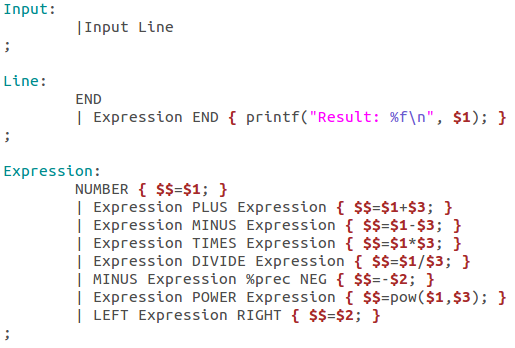
\includegraphics[scale=0.5]{EBNF.png} %A figura pra ser add assim tem q ta no diretorio do tex
            \end{figure} 
\end{frame}


%Slide 18 - Inicio
\begin{frame}
\frametitle{Árvore Sintática da Calculadora }

Exemplos:

\\ 1
\\ 1+3
\\ 1+3*4
\\ 1+3*4-2

\end{frame}

%SLide extra - Inicio
\begin {frame}
\frametitle{Árvore Sintática da Calculadora }
Derivando 1

\begin{figure} 	%para inserir figura basta fazer o mesmo que frame
            \centering		% Significa que a figura está centralizada no slide
            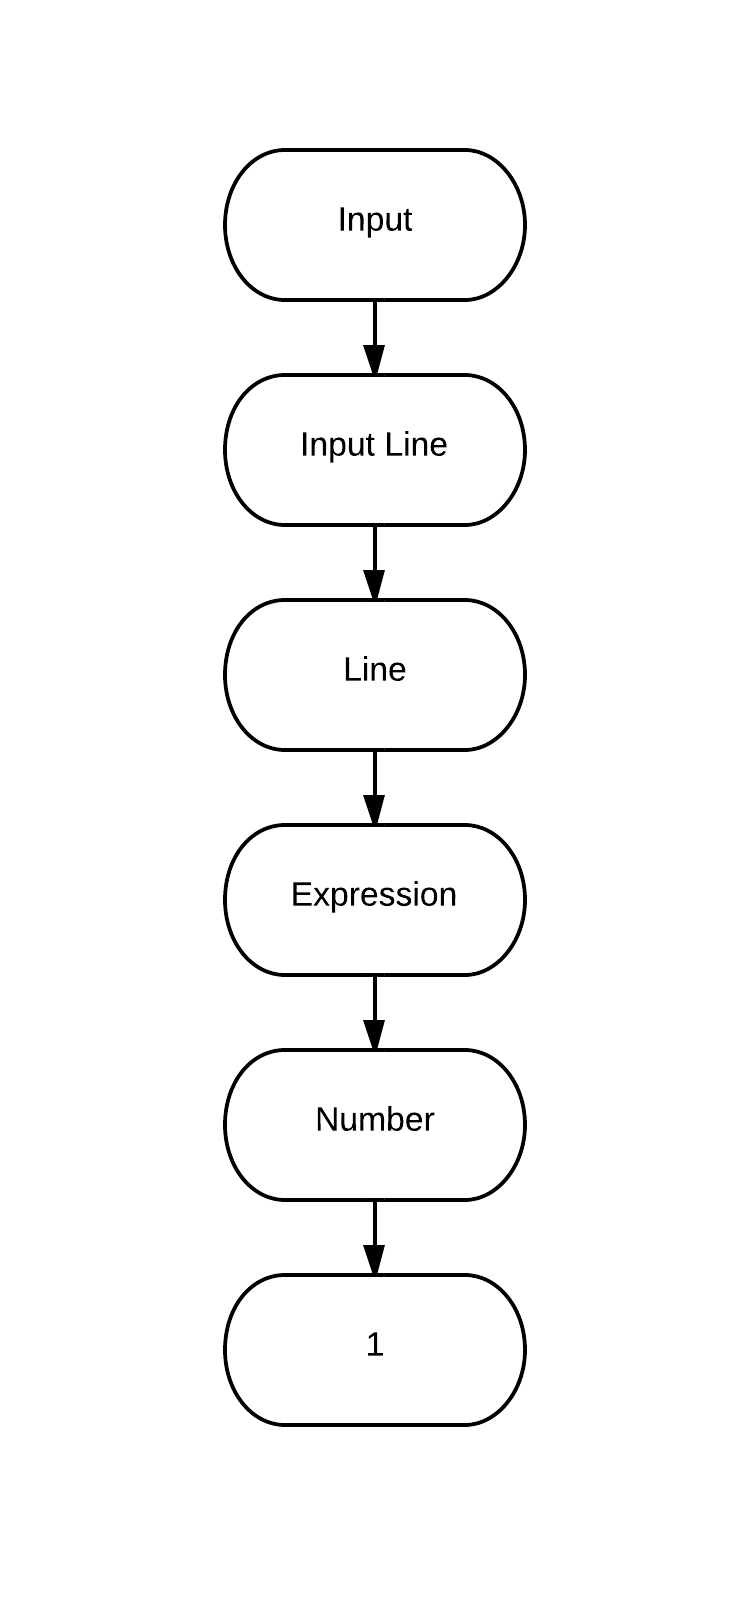
\includegraphics[scale=0.12]{1.png} %A figura pra ser add assim tem q ta no diretorio do tex
            \end{figure} 

\end{frame}

%SLide extra - Inicio
\begin {frame}
\frametitle{Árvore Sintática da Calculadora }
Derivando 1+3

\begin{figure} 	%para inserir figura basta fazer o mesmo que frame
            \centering		% Significa que a figura está centralizada no slide
            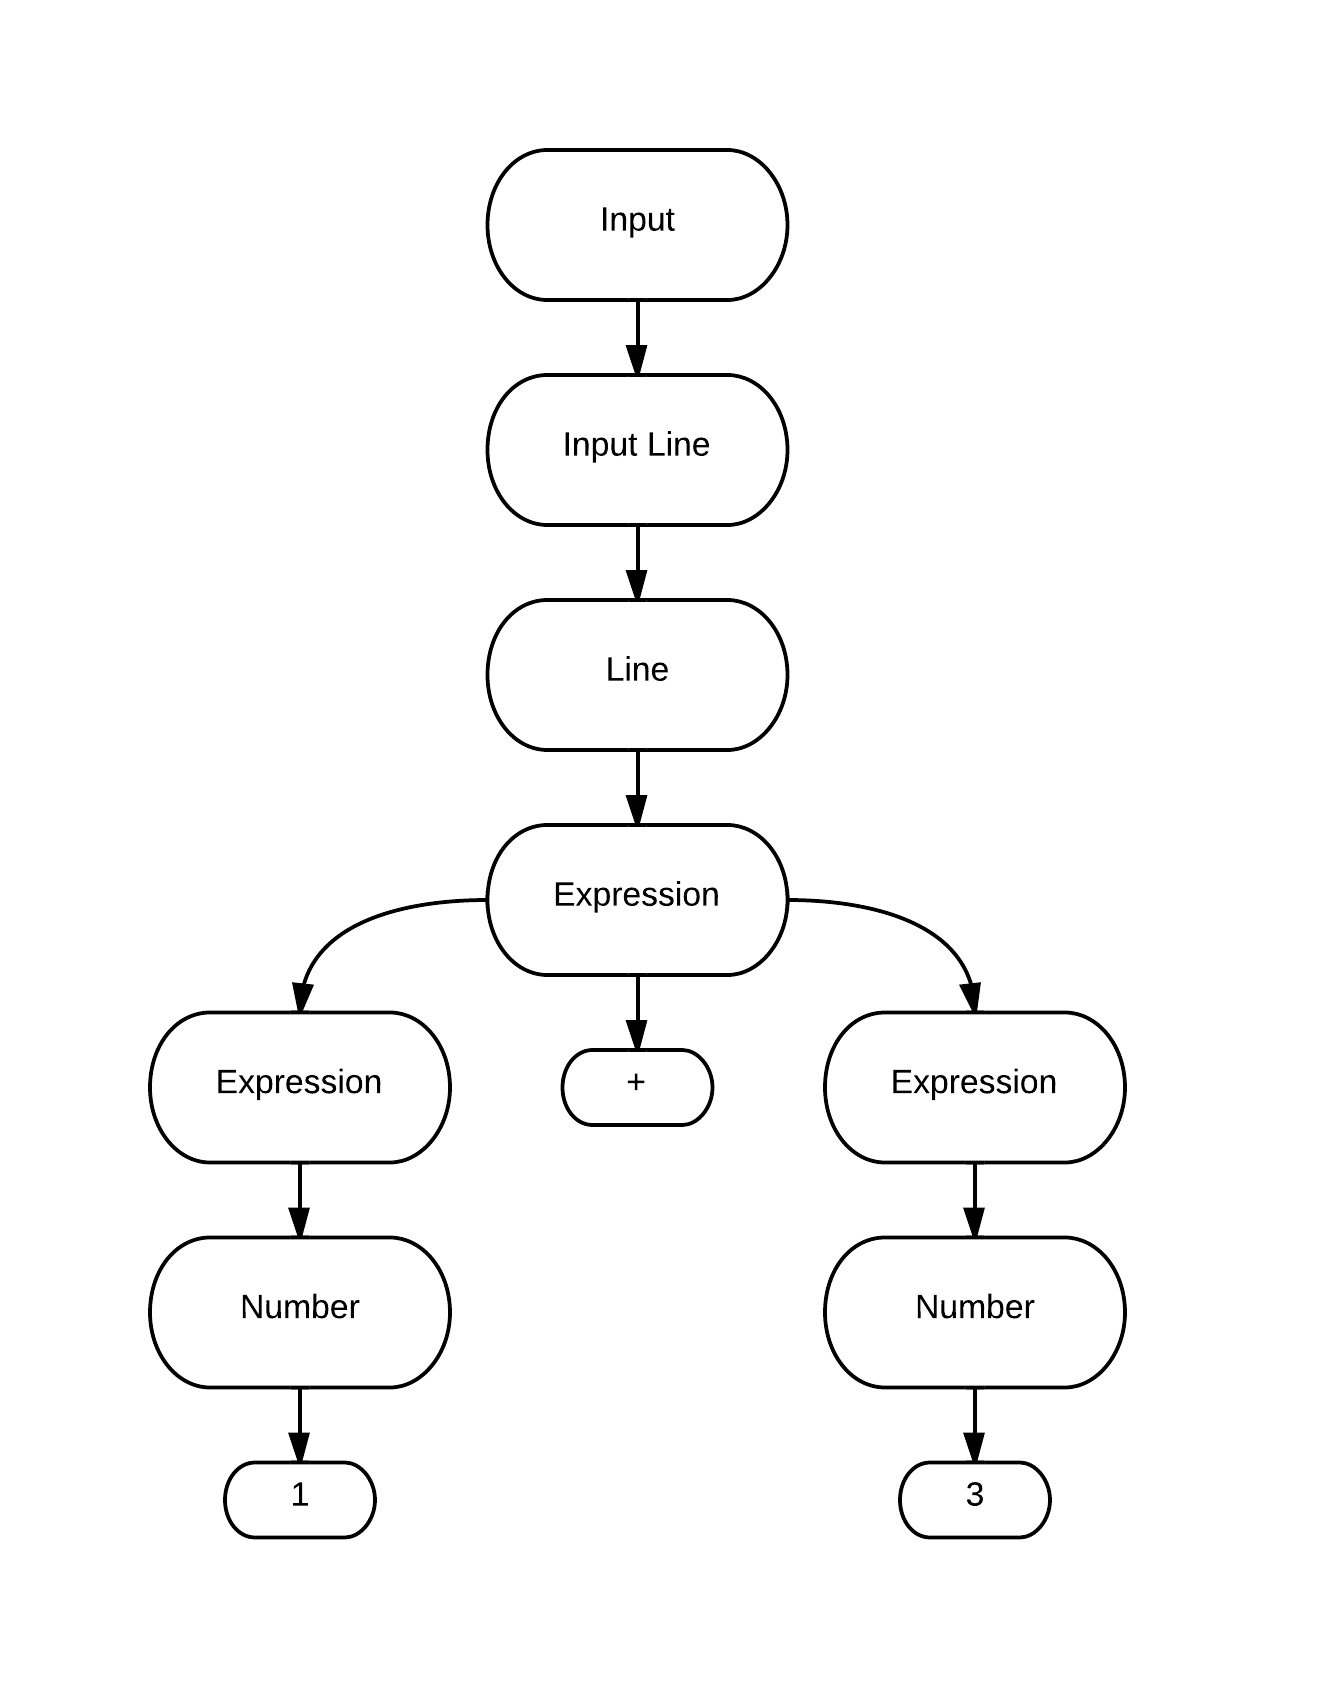
\includegraphics[scale=0.12]{2.png} %A figura pra ser add assim tem q ta no diretorio do tex
            \end{figure} 

\end{frame}

%SLide extra - Inicio
\begin {frame}
\frametitle{Árvore Sintática da Calculadora }
Derivando 1+3*4

\begin{figure} 	%para inserir figura basta fazer o mesmo que frame
            \centering		% Significa que a figura está centralizada no slide
            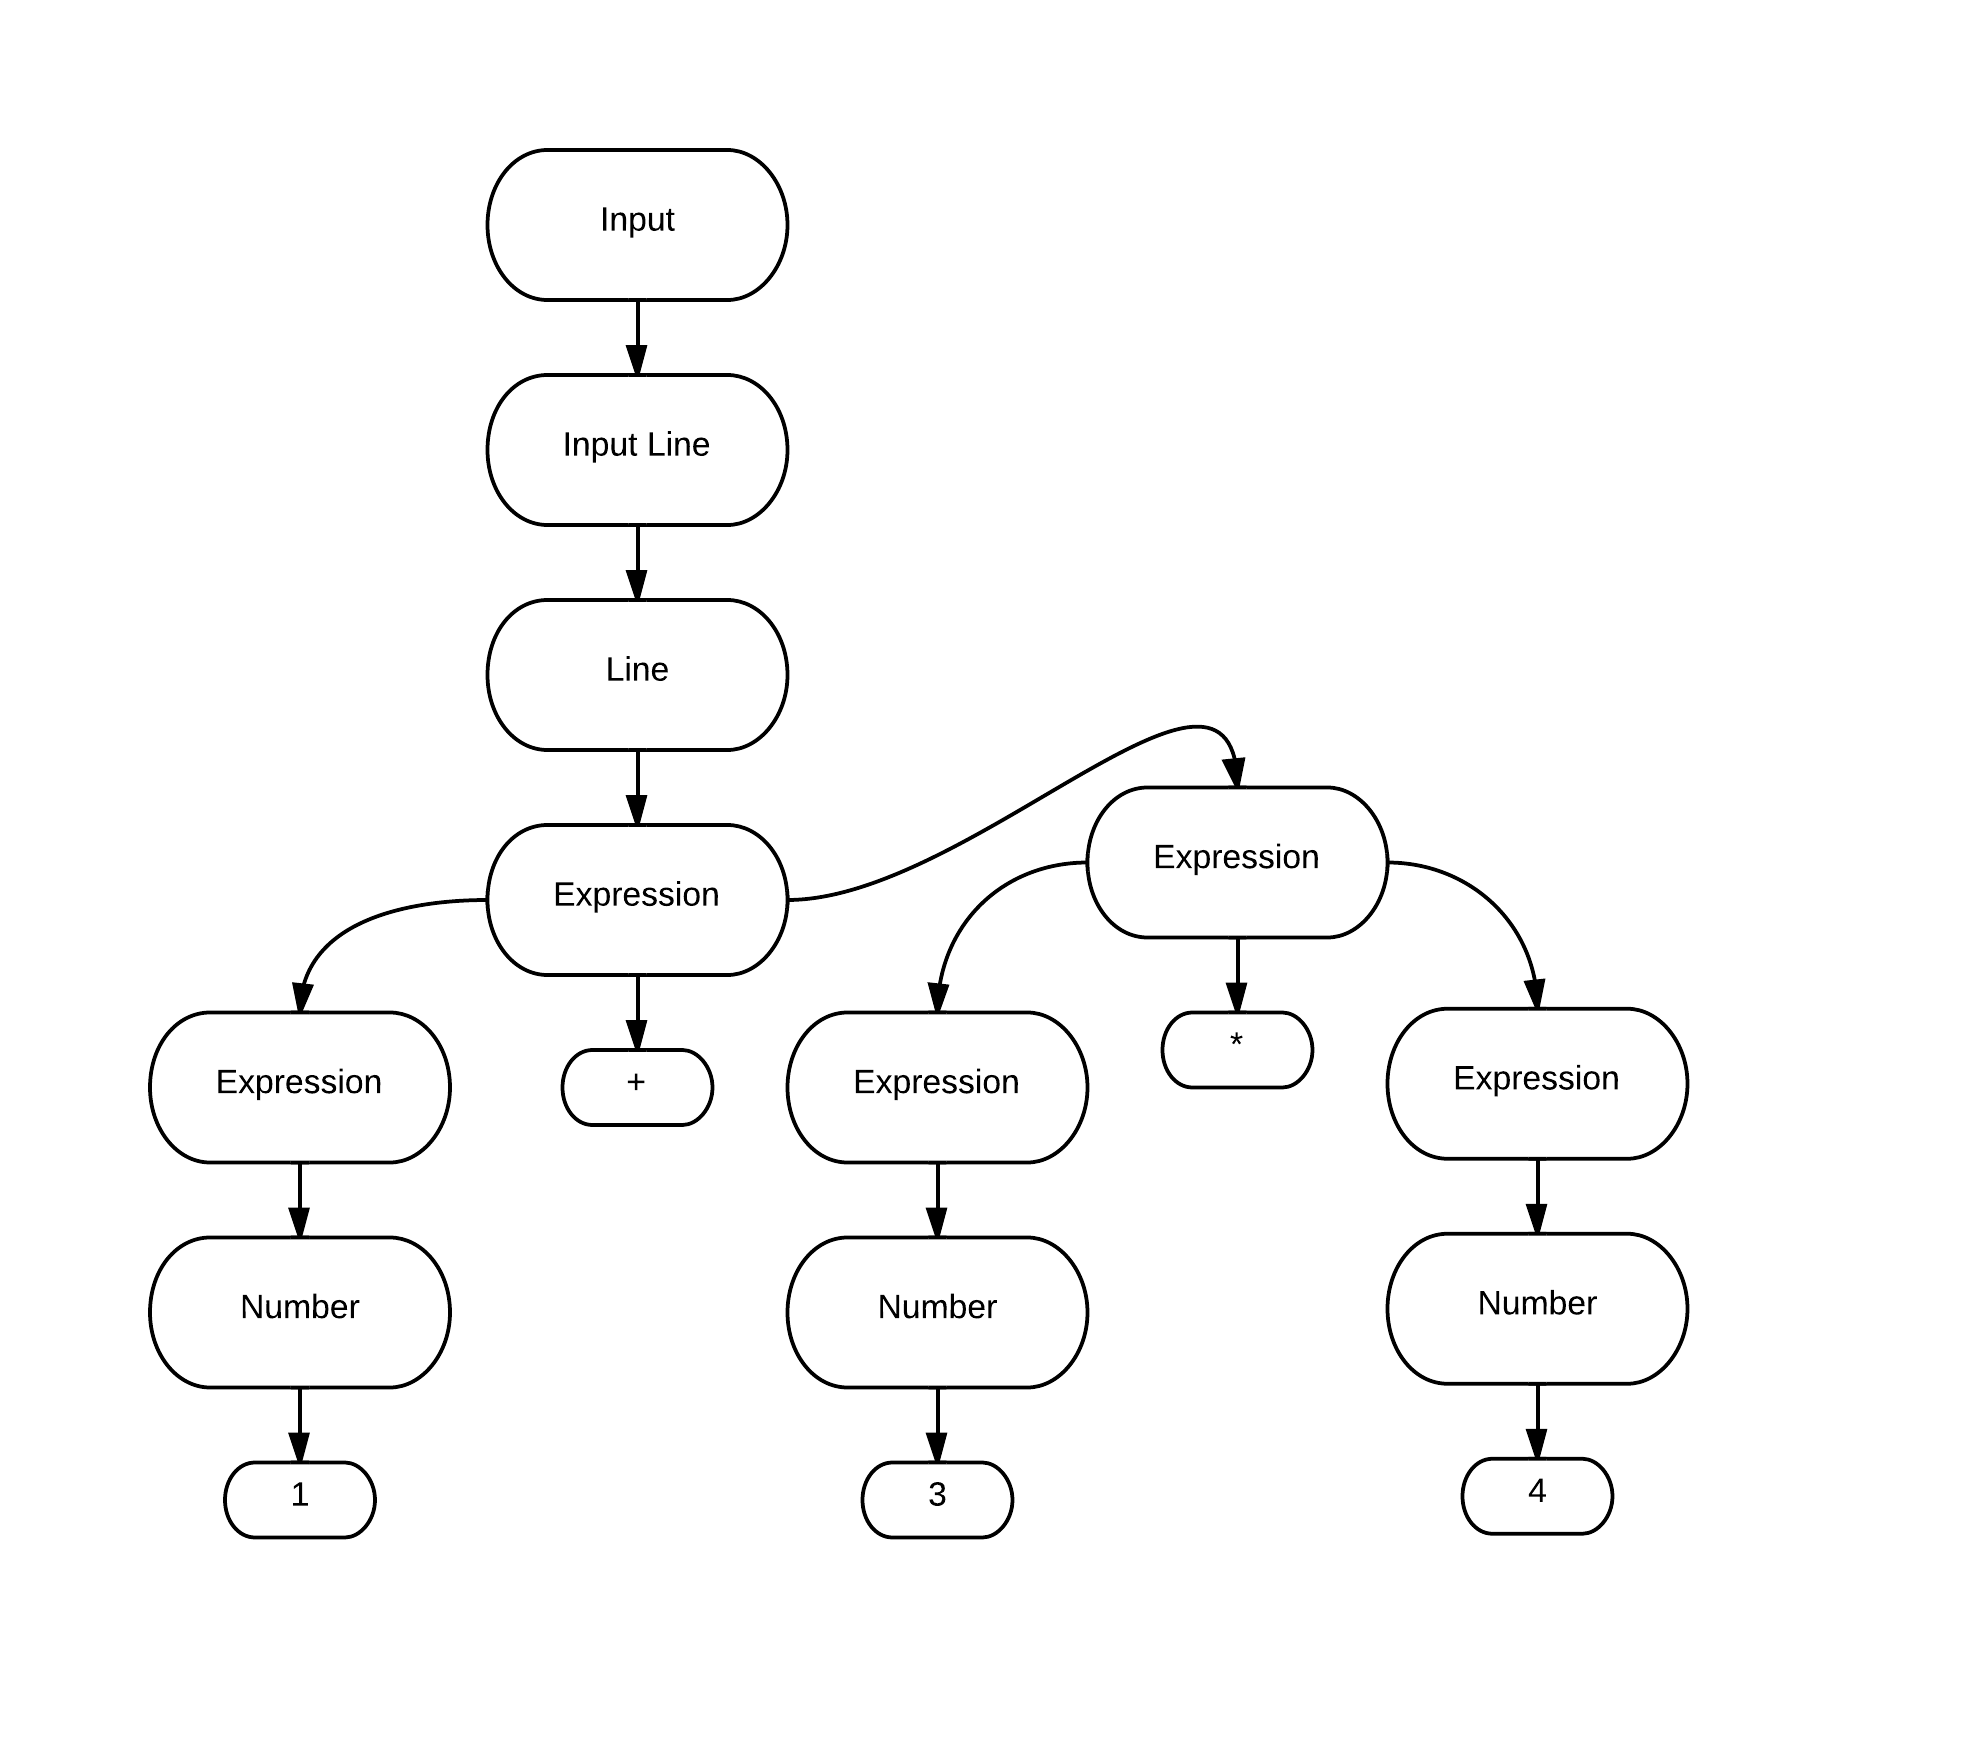
\includegraphics[scale=0.12]{3.png} %A figura pra ser add assim tem q ta no diretorio do tex
            \end{figure} 

\end{frame}

%SLide extra - Inicio
\begin {frame}
\frametitle{Árvore Sintática da Calculadora }
Derivando 1+3*4-2

\begin{figure} 	%para inserir figura basta fazer o mesmo que frame
            \centering		% Significa que a figura está centralizada no slide
            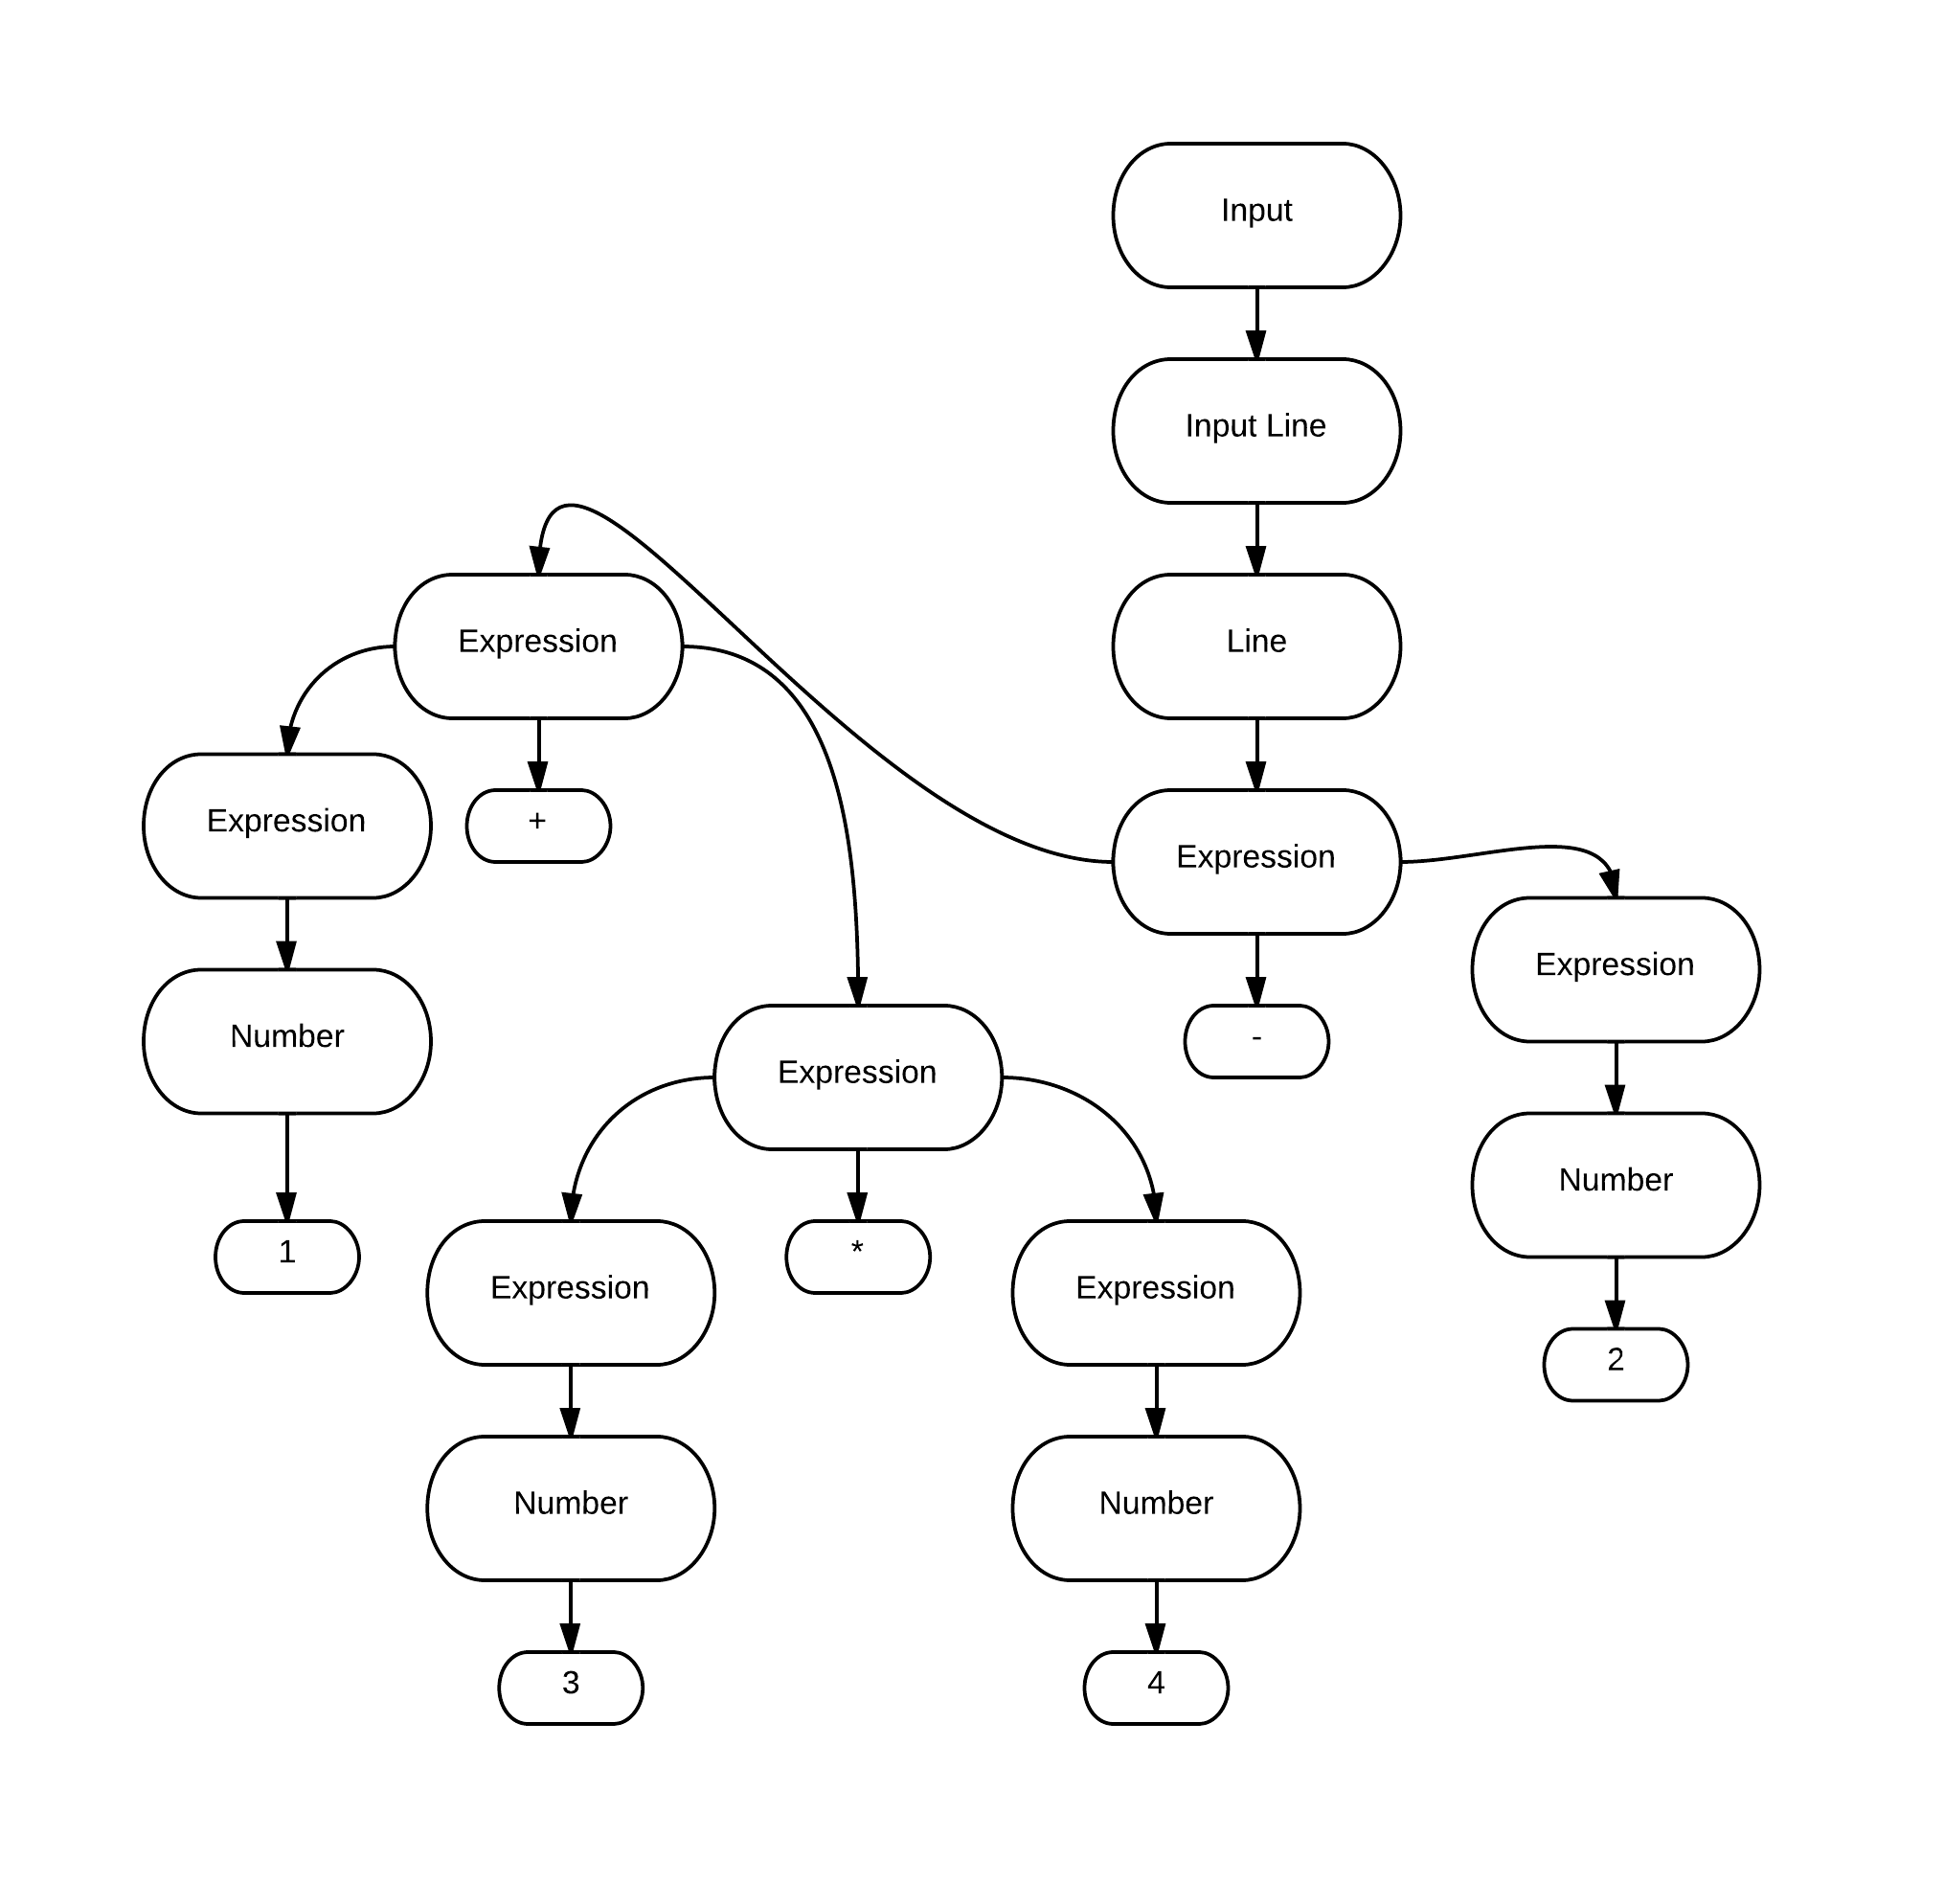
\includegraphics[scale=0.1]{4.png} %A figura pra ser add assim tem q ta no diretorio do tex
            \end{figure} 

\end{frame}


%Slide 19 - Inicio
\begin{frame}
\frametitle{Árvore Sintática da Calculadora }

Expressões com parênteses 

(1+3)*4-2 \\
(1+3)*(4-2) \\
(1+3)*4(-2)

\end{frame}

\begin {frame}
\frametitle{Árvore Sintática da Calculadora }
Derivando (1+3)*4-2

\begin{figure} 	%para inserir figura basta fazer o mesmo que frame
            \centering		% Significa que a figura está centralizada no slide
            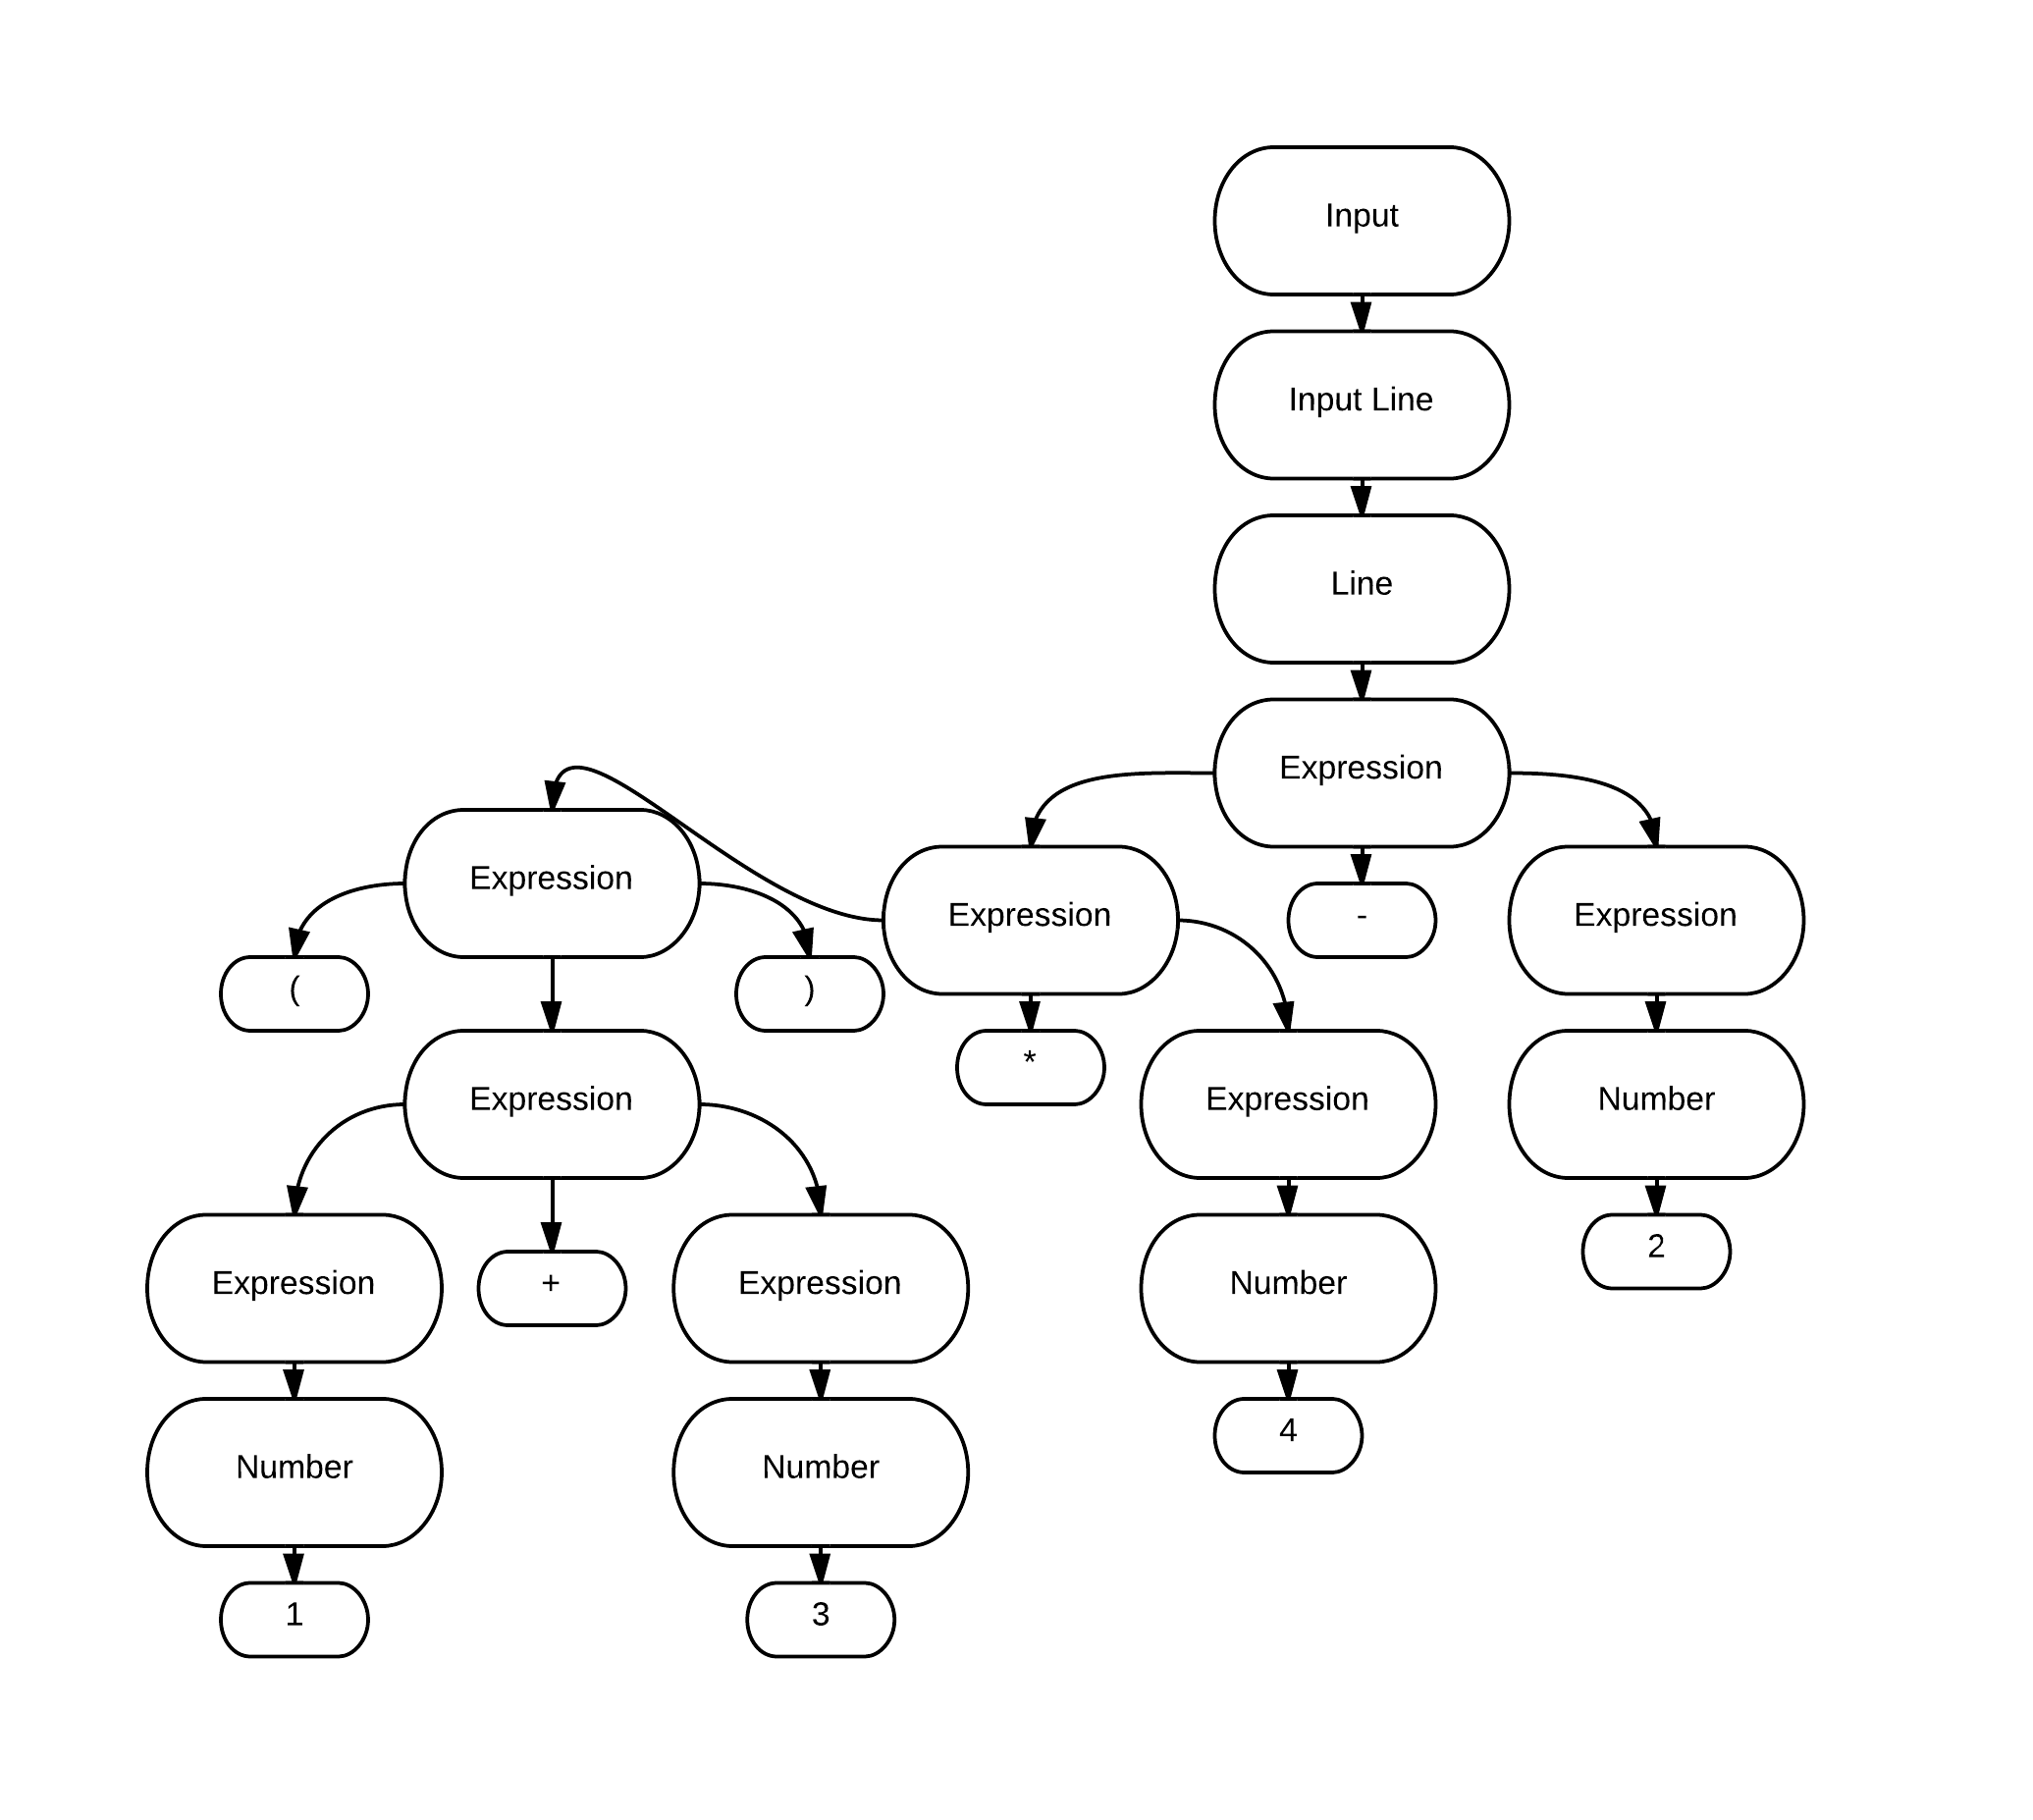
\includegraphics[scale=0.1]{5.png} %A figura pra ser add assim tem q ta no diretorio do tex
            \end{figure} 

\end{frame}

\begin {frame}
\frametitle{Árvore Sintática da Calculadora }
Derivando (1+3)*(4-2)

\begin{figure} 	%para inserir figura basta fazer o mesmo que frame
            \centering		% Significa que a figura está centralizada no slide
            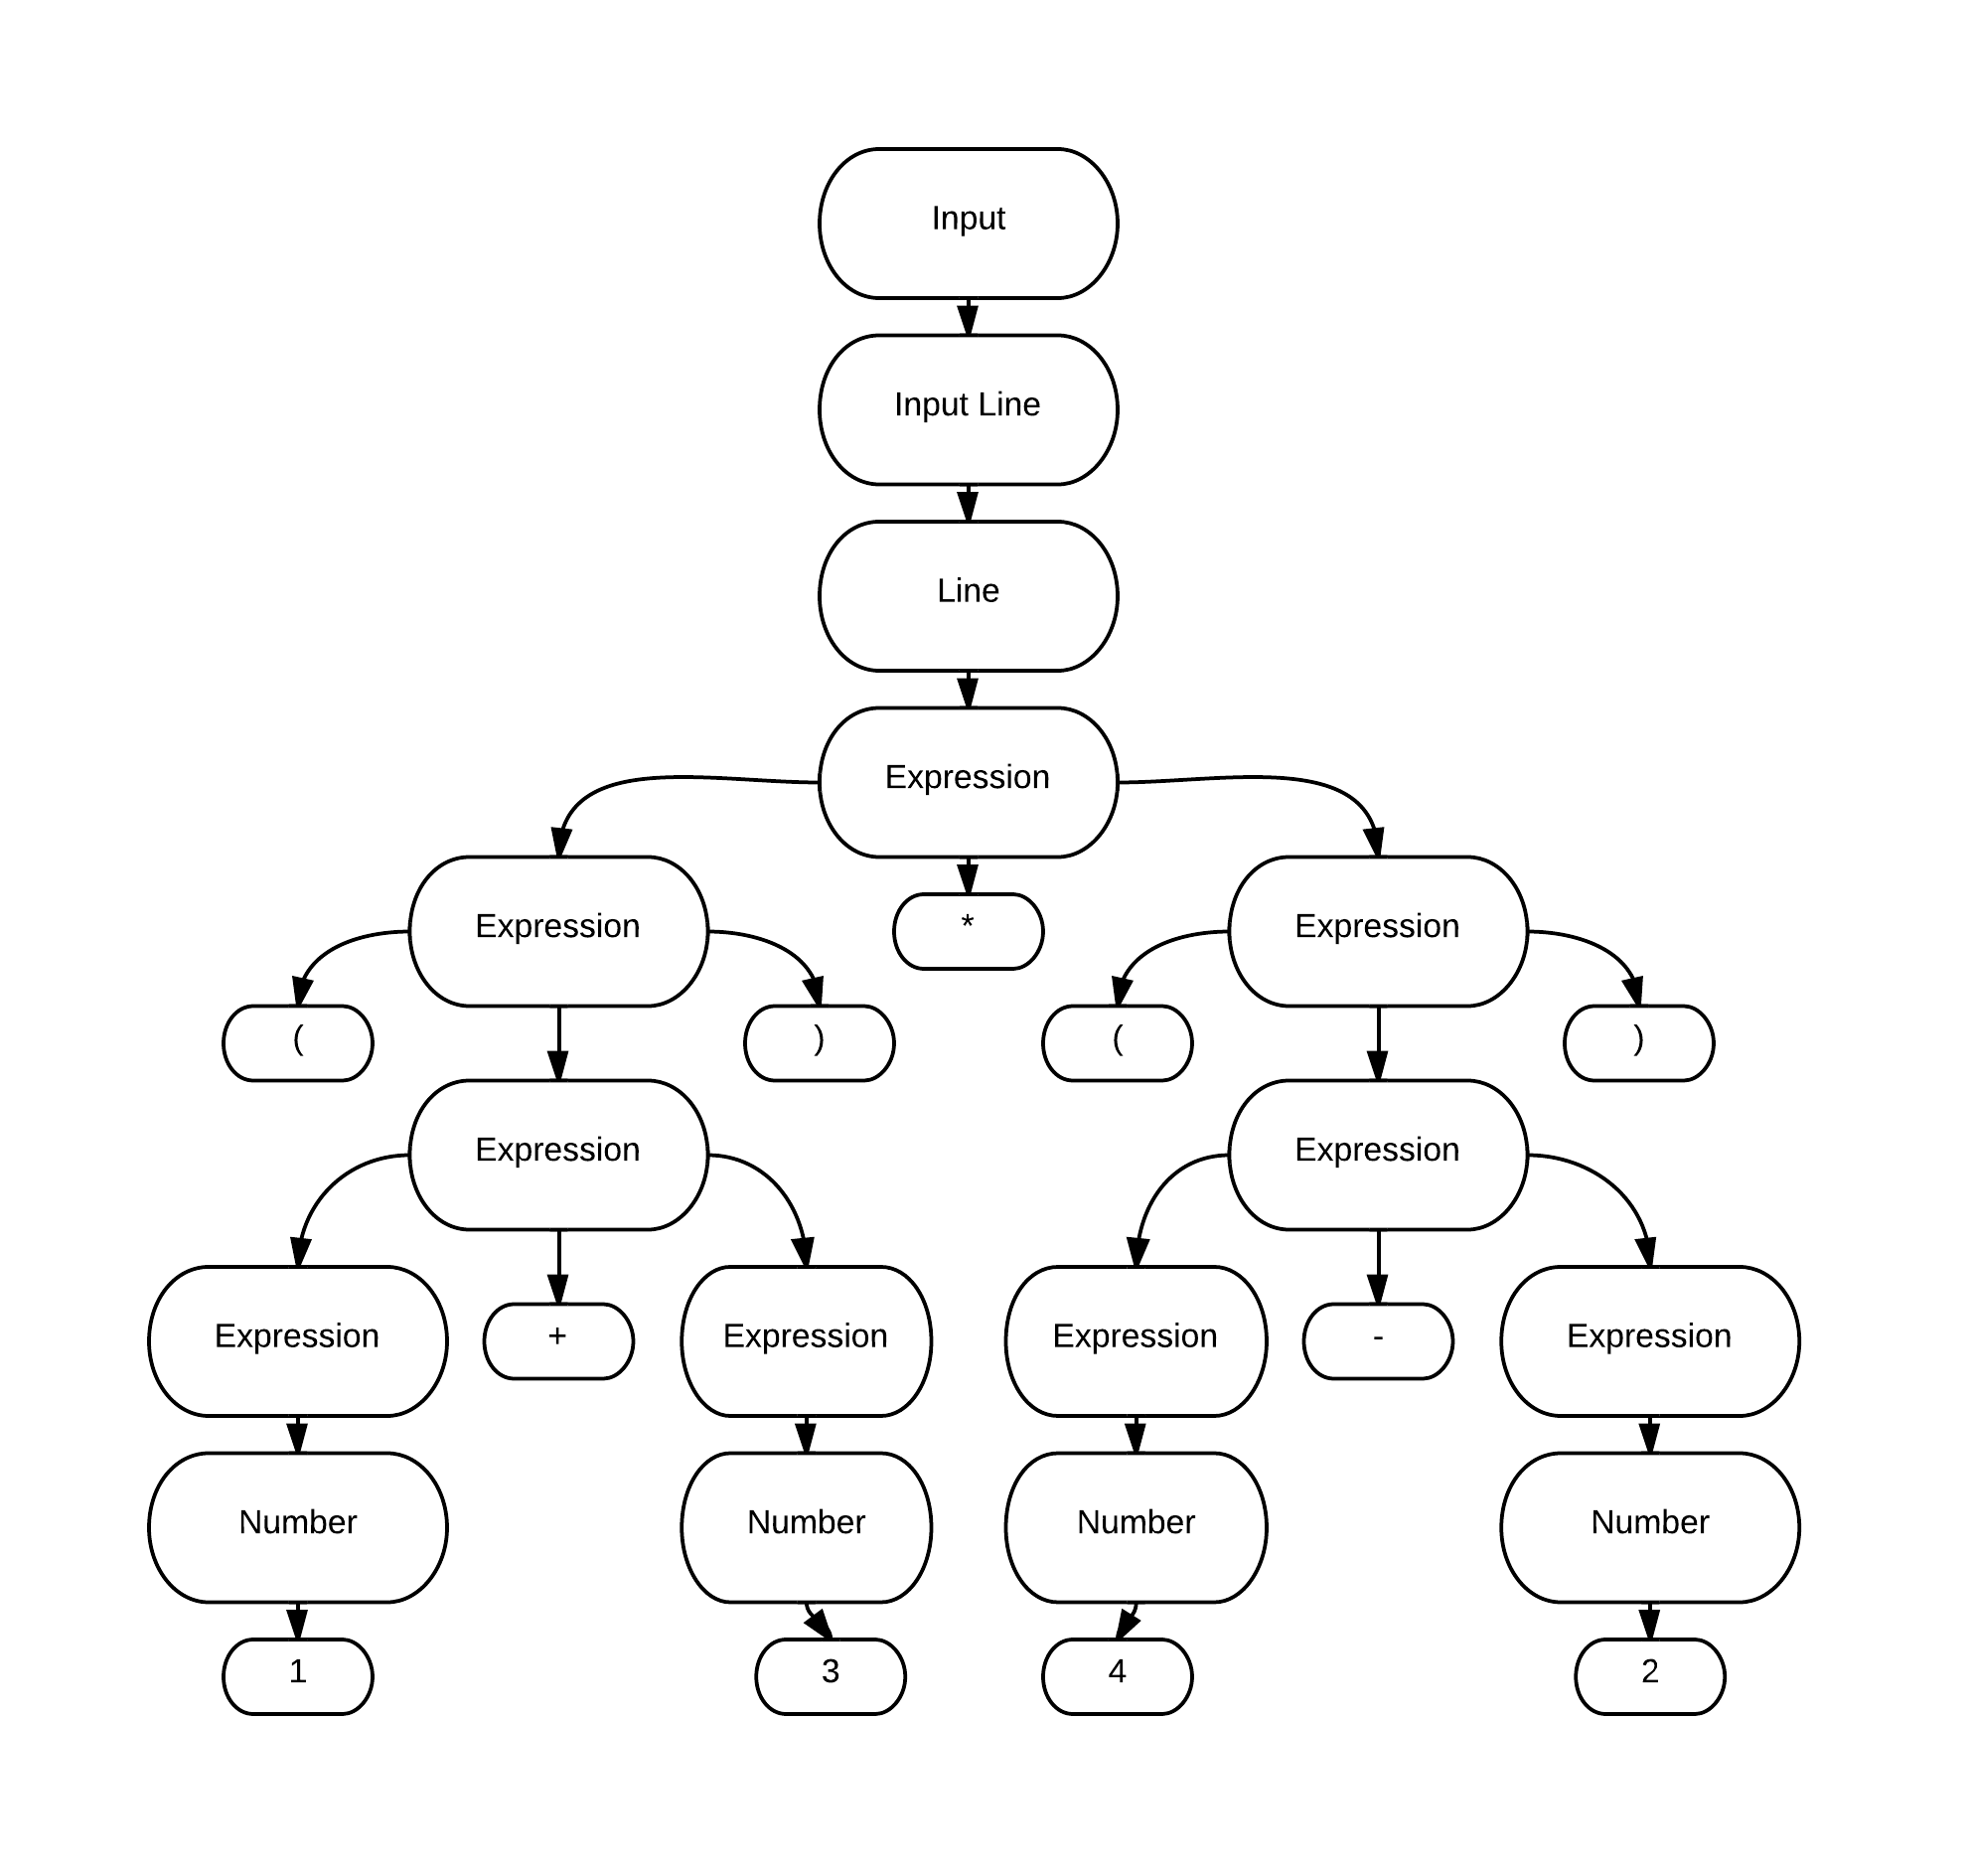
\includegraphics[scale=0.1]{6.png} %A figura pra ser add assim tem q ta no diretorio do tex
            \end{figure} 

\end{frame}

\begin {frame}
\frametitle{Árvore Sintática da Calculadora }
Derivando (1+3)*4(-2) <- ERRO DE SINTAXE

\begin{figure} 	%para inserir figura basta fazer o mesmo que frame
            \centering		% Significa que a figura está centralizada no slide
            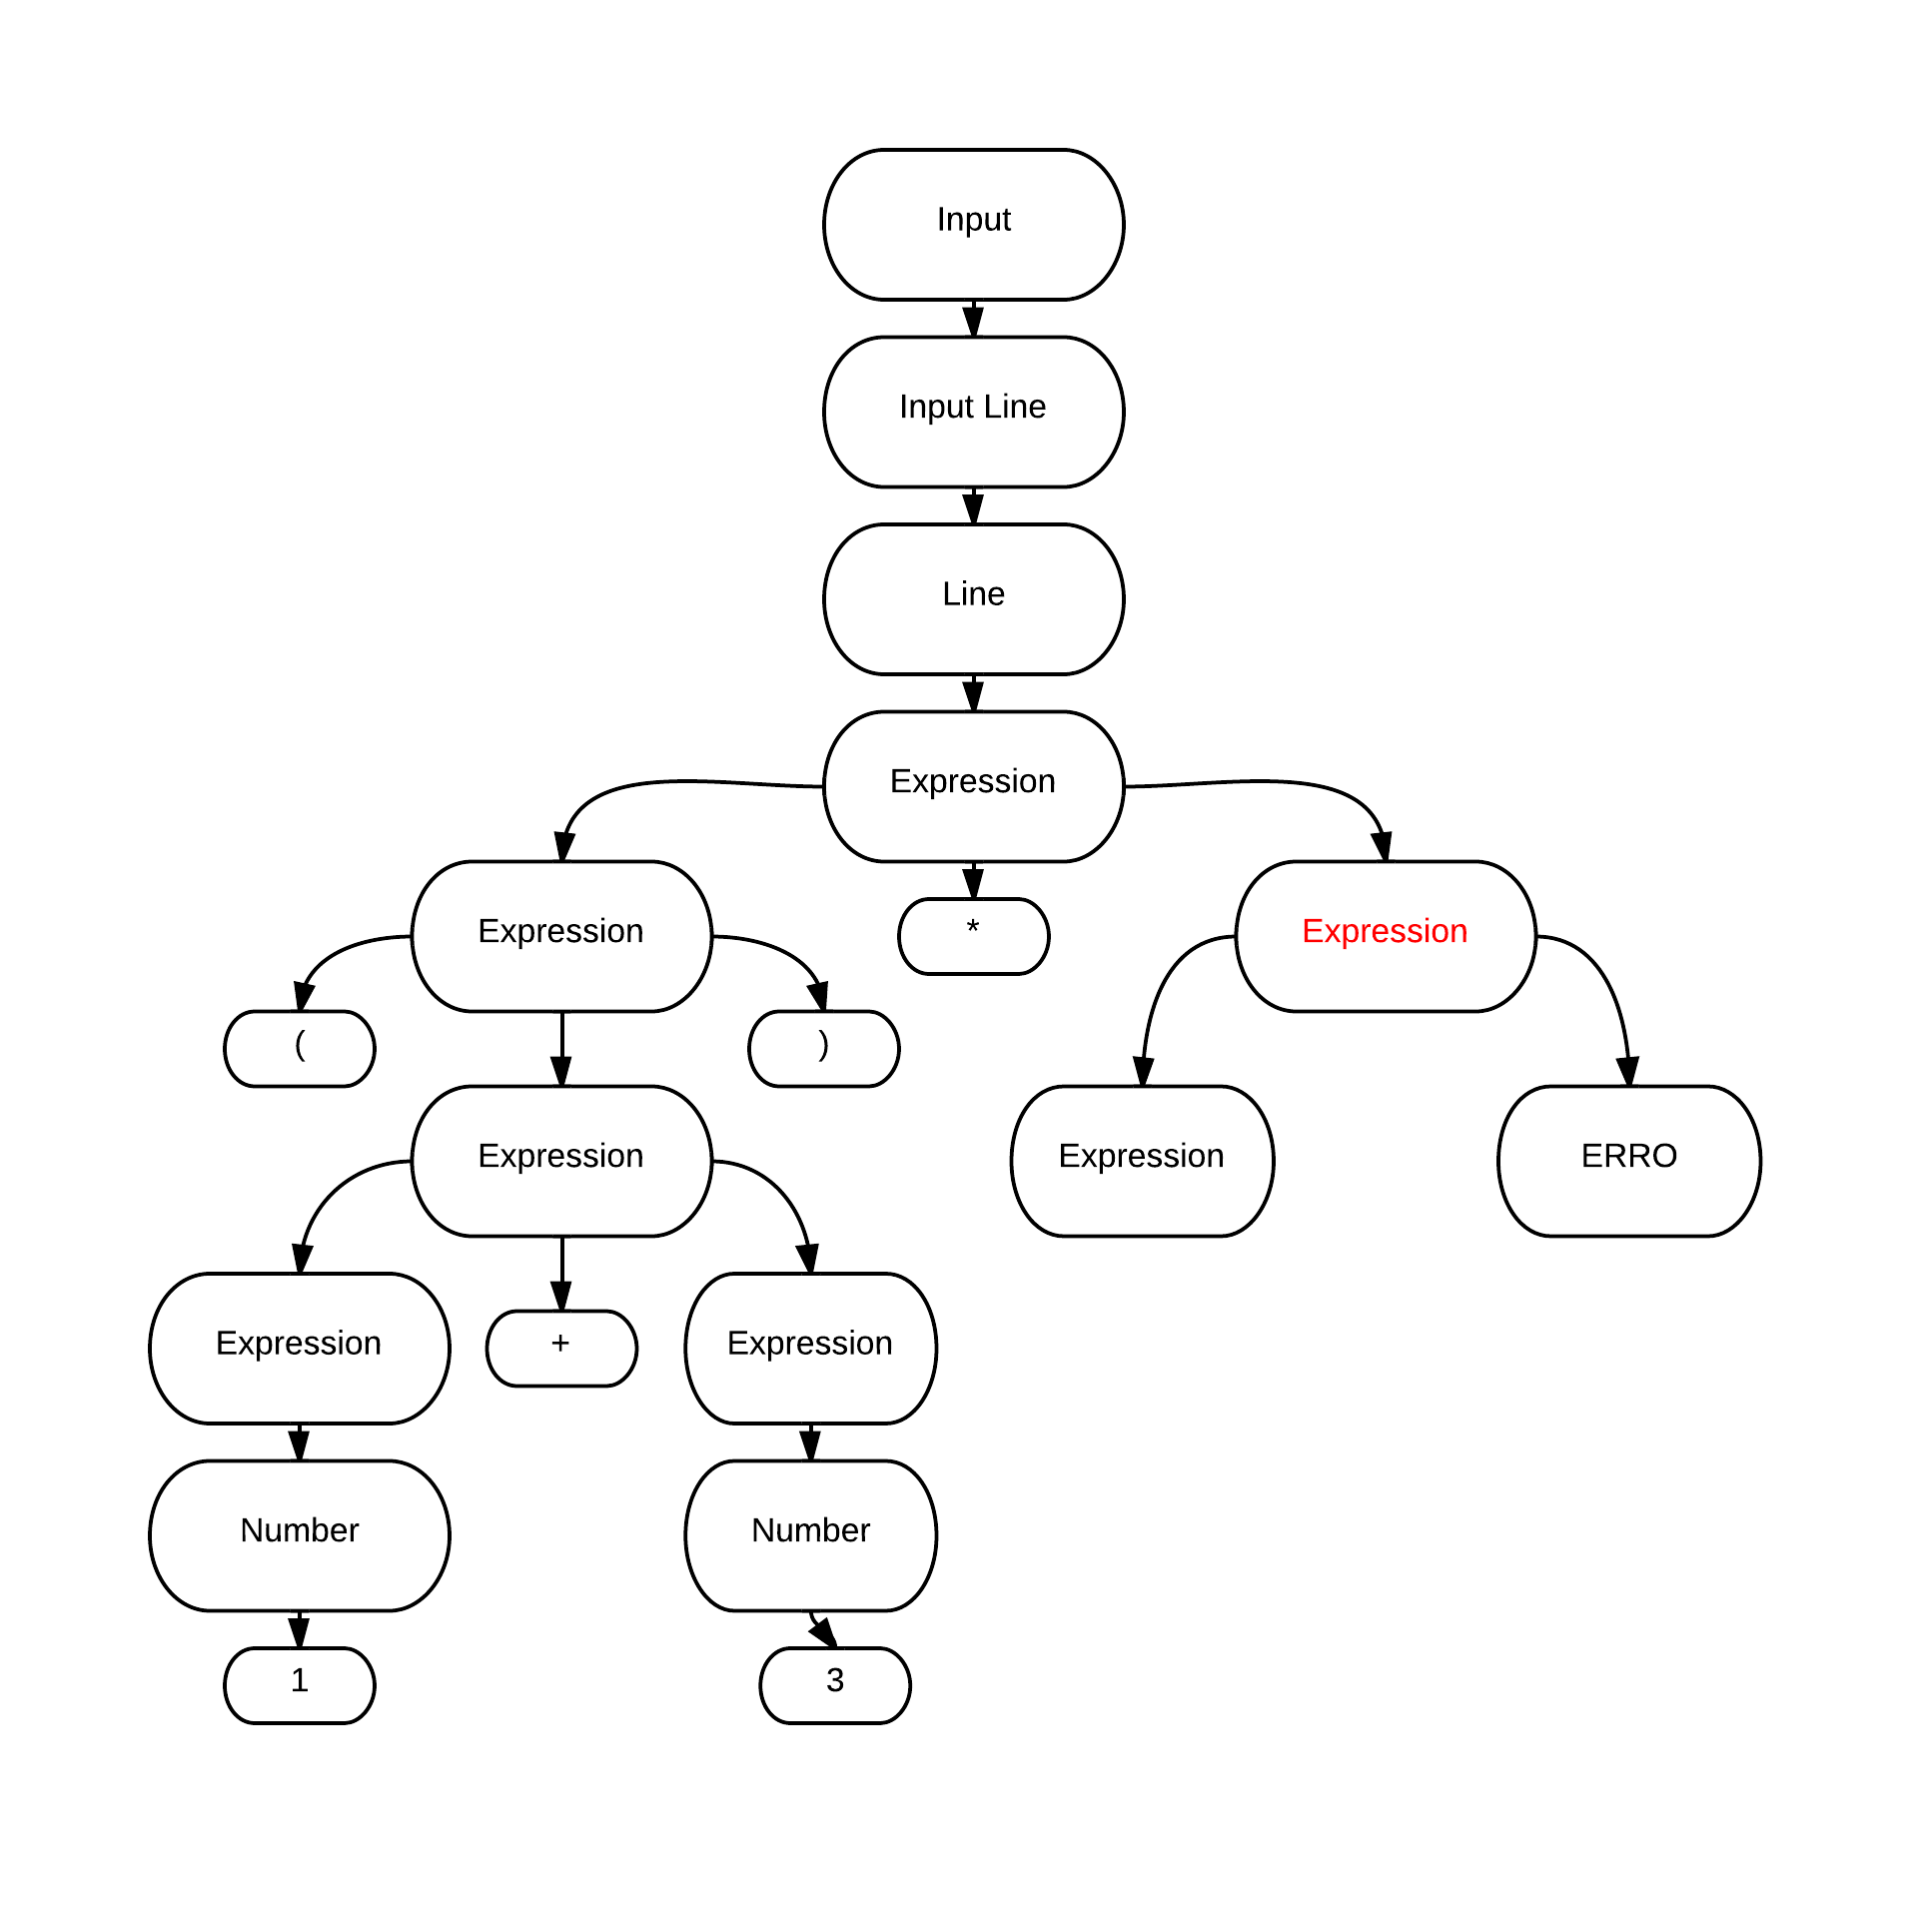
\includegraphics[scale=0.1]{7.png} %A figura pra ser add assim tem q ta no diretorio do tex
            \end{figure} 

\end{frame}



\end{document}





